% ============================================================
% ECONOMICS WORKING-PAPER TEMPLATE  (Tyler Sotomayor house style)
% Preamble and skeleton for the course report; sections live in sections/.
% Build:  ./compile.sh      Audit refs:  ./check_refs.sh --strict
%
% Edit paper_info.tex for title-page metadata. Remaining fill-in points are
% marked % EDIT: -- search for them.
% ============================================================
% LABEL NAMING CONVENTION (enforced by ./check_refs.sh)
% ------------------------------------------------------------
%   sec:<slug>    -- \section, \subsection, \subsubsection
%   app:<slug>    -- appendix sections
%   fig:<slug>    -- figures
%   tab:<slug>    -- tables
%   eq:<slug>     -- numbered equations
%   prop:<slug>   -- propositions / lemmas / corollaries
%   par:<slug>    -- paragraph-level targets (optional)
%
% <slug> uses lowercase-hyphen (e.g., tab:msc-unemp-cat,
% fig:irf-supply, sec:model-sam). No underscores, no
% camelCase. Prefer descriptive slugs over tab:tab1 style.
% ============================================================

\documentclass[11pt]{article}
% Keep the fonts embedded in Stata figure PDFs. Without this, pdfTeX reuses the
% body Latin Modern font for figure text with the same name and drops ligatures.
\pdfinclusioncopyfonts=1

% ---- Layout ----
\usepackage[margin=1in]{geometry}
\usepackage{setspace}
\usepackage{lmodern}
\usepackage[T1]{fontenc}
\usepackage[utf8]{inputenc}

% ---- Paper metadata and title-page content ----
% ============================================================
% Single-author course report metadata, using the working-paper frontmatter.
% ============================================================

\newcommand{\papershorttitle}{Snack Choices and Decision Times}
\newcommand{\paperfulltitle}{Snack Choices and Decision Times under the Drift-Diffusion Model}
\newcommand{\paperauthor}{Tyler Sotomayor}
\newcommand{\paperpdfsubject}{ECON GU4850 Project Report 1}
\newcommand{\paperdate}{October 2026}
\newcommand{\paperyear}{2026}
\newcommand{\paperinstitution}{Columbia University}
\newcommand{\paperdepartment}{Columbia University, Department of Economics}
\newcommand{\papercourse}{ECON GU4850}
\newcommand{\papercoursetitle}{Cognitive Mechanisms \& Economic Behavior}
\newcommand{\paperterm}{Fall 2026}
\newcommand{\paperreport}{Project Report 1}
\newcommand{\paperfulldate}{October 5, 2026}
\newcommand{\paperlatesturl}{https://github.com/tylersotomayor/ddm-snack-choices/blob/main/output/pdf/project-1-report.pdf}
\newcommand{\paperlatesttext}{github.com/tylersotomayor/ddm-snack-choices}
\newcommand{\paperrepourl}{https://github.com/tylersotomayor/ddm-snack-choices}
\newcommand{\paperreplicationurl}{https://github.com/tylersotomayor/ddm-snack-choices/tree/main/replication/project-1-replication}
\newcommand{\paperreplicationtext}{github.com/tylersotomayor/ddm-snack-choices/tree/main/replication}

\title{\huge\bfseries Snack Choices and Decision Times%
  \\[0.3em] under the Drift-Diffusion Model%
  \thanks{Prepared for ECON GU4850, Cognitive Mechanisms and Economic Behavior,
  Columbia University. I thank Michael Woodford and Andrew Souther for helpful
  discussions and guidance. UNI: ts3686. October 5, 2026.
  \S~Corresponding author:
  \href{mailto:tyler.sotomayor@columbia.edu}{tyler.sotomayor@columbia.edu}.
  Please cite as: Sotomayor, Tyler (\paperyear).
  ``\paperfulltitle.''
  Project Report 1, \paperinstitution. Latest version:
  \href{\paperlatesturl}{\nolinkurl{\paperlatesttext}}.
  Code and replication package:
  \href{\paperreplicationurl}{\nolinkurl{\paperreplicationtext}}.}}

\author{%
  \vspace{-1.2em}\\
  {\Large
  \href{https://tylersotomayor.com}{\paperauthor}\textsuperscript{\S}}
  \\[1.5em]
  {\Large \paperinstitution} \\[1.5em]
  {\normalsize \paperreport} \\[0.6em]
  {\normalsize \paperfulldate}
}

\date{\vspace{-3em}}

\newcommand{\AlphaIndividual}{0.408}
\newcommand{\AlphaPooled}{0.308}
\newcommand{\LLIndividual}{ -192.61}
\newcommand{\LLPooled}{-14{,}580.86}
\newcommand{\TimeScaleIndividual}{ 2913}
\newcommand{\OffsetIndividual}{ 644}
\newcommand{\TimeScalePooled}{ 2657}
\newcommand{\OffsetPooled}{ 539}
\newcommand{\RSquaredIndividual}{0.554}
\newcommand{\RSquaredPooled}{0.961}
\newcommand{\RTMean}{ 1,892}
\newcommand{\RTSD}{ 1,728}
\newcommand{\RTLower}{-1562.61}
\newcommand{\RTUpper}{ 5347.44}
\newcommand{\RTKept}{418}
\newcommand{\RTRemoved}{ 17}
\newcommand{\MaxDelta}{4.67}
\newcommand{\BinWidth}{0.622}
\newcommand{\ChoiceRMSEIndividual}{ 6.7}
\newcommand{\ChoiceRMSEPooled}{ 3.6}
\newcommand{\RTRMSEIndividual}{ 172}
\newcommand{\RTRMSEPooled}{  37}
\newcommand{\CurveGapIndividual}{ 2.7}
\newcommand{\AltAIndividual}{ 2917}
\newcommand{\AltOffsetIndividual}{ 643}
\newcommand{\AltRSquaredIndividual}{0.555}


% ---- Math ----
\usepackage{amsmath, amssymb, amsthm}

% ---- Theorem environments ----
\newtheorem{proposition}{Proposition}
\newtheorem{corollary}[proposition]{Corollary}
\newtheorem{lemma}[proposition]{Lemma}
\newtheorem{assumption}{Assumption}
\newtheorem{definition}{Definition}

% ---- Tables and Figures ----
\usepackage{graphicx}
\usepackage{booktabs}
\usepackage{float}
\usepackage[
  font=small,
  labelfont=sc,
  textfont=sc,
  labelsep=colon,
  justification=centering
]{caption}

% ---- Lists and Formatting ----
\usepackage{enumitem}
\usepackage{titlesec}
\usepackage[strings]{underscore}

% ---- Page headers ----
\usepackage{fancyhdr}
\pagestyle{fancy}
\fancyhf{}
\renewcommand{\headrulewidth}{0pt}
\fancyhead[C]{\small\itshape \papershorttitle}
\fancyfoot[C]{\thepage}

% ---- Section styling ----
\setcounter{secnumdepth}{1}
\setcounter{tocdepth}{2}

\titleformat{\section}{\LARGE\bfseries}{\thesection}{1em}{}
\titlespacing*{\section}{0pt}{1.5em}{0.8em}

\titleformat{\subsection}[runin]{\normalfont\bfseries}{}{0pt}{}[.]
\titlespacing*{\subsection}{0pt}{1em}{0.5em}

\titleformat{\subsubsection}[runin]{\normalfont\bfseries\itshape}{}{0pt}{}[.]
\titlespacing*{\subsubsection}{0pt}{0.8em}{0.5em}

\titleformat{\paragraph}[runin]{\bfseries}{}{0pt}{}[.]
\titlespacing*{\paragraph}{0pt}{0.8em}{0.5em}

% ---- Diagrams ----
\usepackage{tikz}

% ---- Bibliography ----
\usepackage[style=apa, backend=biber]{biblatex}
\DeclareLanguageMapping{american}{american-apa}
\addbibresource{literature/references.bib}

\AtBeginBibliography{%
  \renewcommand*{\mkbibnamefamily}[1]{\textsc{\lowercase{#1}}}%
  \renewcommand*{\mkbibnamegiven}[1]{#1}%
  \renewcommand*{\mkbibnameprefix}[1]{#1}%
  \renewcommand*{\mkbibnamesuffix}[1]{#1}%
}

% ---- Colors ----
\usepackage{xcolor}

% ---- Hyperlinks ----
\usepackage{hyperref}
\hypersetup{
  pdftitle={\paperfulltitle},
  pdfauthor={\paperauthor},
  pdfsubject={\paperpdfsubject},
  colorlinks=true,
  linkcolor=black,
  citecolor=black,
  urlcolor=black
}

% ---- Course banner overlay ----
\usepackage{eso-pic}

% ---- Paths ----
\graphicspath{{output/figures/}}
\providecommand{\sym}[1]{\ifmmode^{#1}\else\(^{#1}\)\fi}
\newcommand{\capttitle}[1]{#1}
\newcommand{\floatnotes}[1]{%
  \par\vspace{0.35em}%
  \begin{minipage}{0.94\linewidth}%
    \footnotesize\raggedright\textit{Notes:} #1%
  \end{minipage}\par%
}

% ---- Formatting ----
\setlength{\parindent}{1.5em}
\setlength{\parskip}{0pt}

% ---- Appendix numbering ----
\newcommand{\appendixnumbering}{%
  \setcounter{table}{0}%
  \renewcommand{\thetable}{A\arabic{table}}%
  \setcounter{figure}{0}%
  \renewcommand{\thefigure}{A\arabic{figure}}%
}

% ---- Course banner ----
\newcommand{\workingpaperheader}{%
\AddToShipoutPictureFG*{%
  \AtPageUpperLeft{%
    \hspace*{0pt}%
    \raisebox{-1.10in}{%
      \parbox{\paperwidth}{%
        \centering
        {\small\bfseries \papercourse} \enspace{\small\textbar} \enspace{\small \papercoursetitle} \enspace{\small\textbar} \enspace{\small \paperterm}\\[0.1em]
        {\scriptsize \paperdepartment}\\[0.05em]
        \rule{0.5\paperwidth}{0.4pt}%
      }%
    }%
  }%
}%
}

% ============================================================
\begin{document}
% ============================================================

\workingpaperheader

\begingroup
\onehalfspacing
\maketitle

\vspace{1em}

\begin{abstract}
\noindent I estimate a drift-diffusion model of snack choices in Experiment 1,
using differences in bids to measure relative value. My 435 choices yield a
choice-sensitivity estimate of 0.408, compared with 0.308 for the 30,450 choices
pooled across the class. The fitted probabilities rise with the bid difference
in both samples. Pooled choices change more sharply near equal bids and remain
less extreme in the tails than the fitted curve predicts. Response times
provide a second check because their shape depends on the same choice
parameter. Holding that estimate fixed, I fit the time scale and nondecision
time to 15 bin averages. The model explains 55.4 percent of the variation
across my trimmed response-time means and 96.1 percent across the class means.
The class averages follow the predicted inverted-U closely. My data show a
less regular pattern, including faster choices near equal bids than in some
neighboring bins.
\end{abstract}

\vspace{1em}
\noindent \textbf{JEL Codes:} D81, D87

\vspace{0.25em}
\noindent \textbf{Keywords:} drift-diffusion model, stochastic choice, response time


\endgroup

\doublespacing
\newpage

\tableofcontents
\newpage

% ============================================================
%  BODY  (order here controls the section order in the PDF)
% ============================================================

\section{Introduction}
\label{sec:introduction}

Choosing between two similarly valued snacks should take longer than choosing
between a favorite and a much less valued alternative. The drift-diffusion
model (DDM) links this prediction to the probability of choosing each good.
When values are close, evidence drifts slowly toward either decision threshold;
with a larger value difference, choices become more predictable and quicker on
average. I use the formulation presented by
\textcite[slides 10--11 and 24--26]{woodford2026ddm} in Lecture 5.

The individual file, \texttt{indv-Data.csv}, records 435 choices under my UNI,
\texttt{ts3686}. The pooled file,
\texttt{popData.csv}, supplies 15 class bins.
The first good in each individual record is treated as the left good and the
second as the right good. Their mean bids from Section 1 of the experiment
give $v_L$ and $v_R$, so the value difference is $\Delta=v_R-v_L$.
There are 368 distinct pairs of goods, some of which I encountered more than
once; each choice is a separate trial.


\section{Individual Choices}
\label{sec:individual-choices}

\subsection{Choice Probabilities (1a)}
With symmetric thresholds and an unbiased starting point, the model in
\textcite[slide 10]{woodford2026ddm} gives
\begin{equation}\label{eq:choice-probability}
  P_\alpha(\Delta)
  \;=\; \frac{e^{\alpha\Delta}}{e^{\alpha\Delta}+e^{-\alpha\Delta}}
  \;=\; \frac{1}{1+e^{-2\alpha\Delta}}, \qquad \alpha>0.
\end{equation}
The parameter $\alpha$ measures how strongly choices respond to the bid
difference. Since the two possible responses are exhaustive,
\[
  \Pr(L\mid\Delta)
  \;=\; 1-P_\alpha(\Delta)
  \;=\; \frac{e^{-\alpha\Delta}}{e^{\alpha\Delta}+e^{-\alpha\Delta}}
  \;=\; P_\alpha(-\Delta).
\]
Equal values imply a one-half probability of either response, and
reversing the value difference reverses the choice probabilities.

\subsection{Likelihood (1b)}
Let $y_i=1$ if I choose the right good and $y_i=0$ otherwise, and define
$\sigma_i=2y_i-1$. Conditional on the observed bid differences and independent
trial disturbances, the probability of the recorded sequence is
\[
  L(\alpha)
  \;=\; \prod_{i=1}^{435}
       P_\alpha(\Delta_i)^{y_i}
       [1-P_\alpha(\Delta_i)]^{1-y_i}
  \;=\; \prod_{i=1}^{435}P_\alpha(\sigma_i\Delta_i).
\]
Taking logs converts the product into a sum, following the likelihood
construction in \textcite[pp.\ 4--5]{souther2026mle}:
\begin{equation}\label{eq:individual-likelihood}
  LL(\alpha)
  \;=\; \sum_{i=1}^{435}\log P_\alpha(\sigma_i\Delta_i)
  \;=\; -\sum_{i=1}^{435}\log\!\left(1+e^{-2\alpha\sigma_i\Delta_i}\right).
\end{equation}

\subsection{Maximum Likelihood Estimate (1c)}
I maximize equation~\eqref{eq:individual-likelihood} using a logistic
regression of $y_i$ on $\Delta_i$ with no intercept. Its slope is $2\alpha$,
so dividing the estimated coefficient by two gives
\[
  \widehat{\alpha}=\AlphaIndividual,
  \qquad LL(\widehat{\alpha})=\LLIndividual.
\]
The score and curvature provide a check on this numerical estimate:
\[
  LL'(\alpha)=2\sum_i\Delta_i[y_i-P_\alpha(\Delta_i)],
  \qquad
  LL''(\alpha)=-4\sum_i\Delta_i^2P_\alpha(\Delta_i)
                         [1-P_\alpha(\Delta_i)].
\]
At the unrounded estimate, $|LL'(\widehat\alpha)|<10^{-6}$.
The second derivative is negative when at least one bid difference is nonzero,
making the positive optimum unique. Under this fit, a one-dollar advantage
for the right good raises its choice probability to about 69 percent.

\subsection{Binned Comparison (1d)}
Let $M=\max_i|\Delta_i|$, about \MaxDelta\ dollars. I divide $[-M,M]$
into 15 equal intervals, each of width $2M/15\approx\BinWidth$ dollars. Intervals include
their left endpoint and exclude their right endpoint, except that the last
also includes $M$. For the set of trials $B_j$ in bin $j$, with
$N_j=|B_j|$, I calculate
\[
  p_j=\frac{1}{N_j}\sum_{i\in B_j}y_i,
  \qquad
  e_j=\frac{1}{N_j}\sum_{i\in B_j}P_{\widehat\alpha}(\Delta_i).
\]
Inverting equation~\eqref{eq:choice-probability} gives the horizontal
coordinate,
\begin{equation}\label{eq:inverse-probability}
  d_j=P_{\widehat\alpha}^{-1}(e_j)
  \;=\;\frac{1}{2\widehat\alpha}
          \log\!\left(\frac{e_j}{1-e_j}\right).
\end{equation}
With this coordinate, $P_{\widehat\alpha}(d_j)=e_j$, so every predicted bin
point lies exactly on the fitted choice curve.

\begin{figure}[!ht]
  \centering
  \caption{\capttitle{Individual Choice Frequencies}}
  \label{fig:individual-choice}
  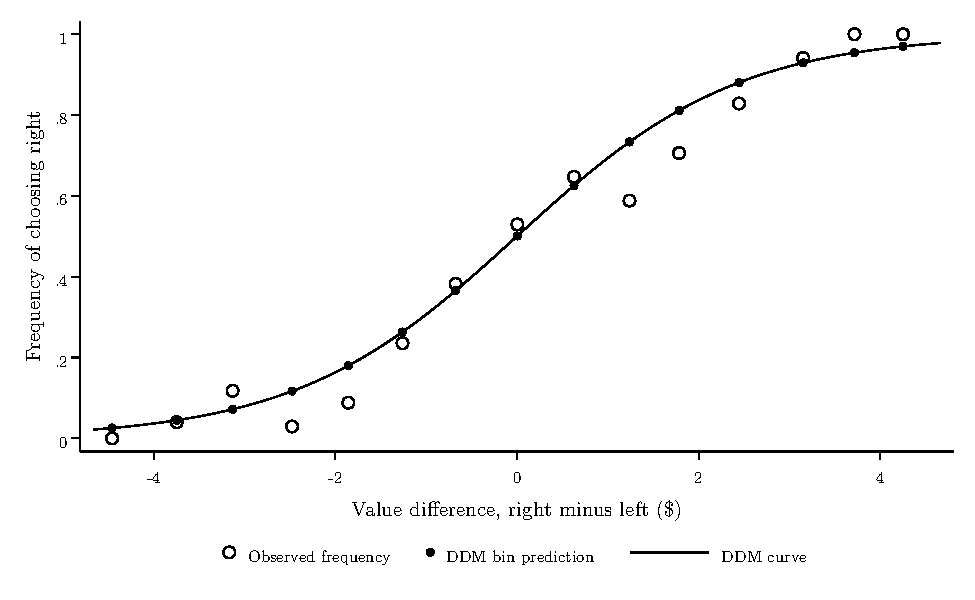
\includegraphics[width=0.94\textwidth]{fig-individual-choice.pdf}
  \floatnotes{Source: \texttt{indv-Data.csv}, UNI \texttt{ts3686}; 435 trials.
  Open circles show observed frequencies $p_j$ in 15 equal-width bins.
  Black dots show mean predicted probabilities $e_j$ at the inverse-probability
  coordinates in equation~\eqref{eq:inverse-probability}. The curve is
  $P_{\widehat\alpha}(d)$, with $\widehat\alpha=\AlphaIndividual$.}
\end{figure}

I almost always chose the higher-bid snack when the bids were far apart
(Figure~\ref{fig:individual-choice}). For nearly equal bids, I chose right in
52.9 percent of trials, close to the predicted 50.1 percent. The intermediate
bins are less regular. Near $d_j=1.24$, the right good won only 20 of 34
choices despite its higher bid, while the model puts its choice probability
at 73.3 percent. In the bin near $d_j=-1.86$, I chose right in 8.8 percent
of trials, roughly half the predicted 18.0 percent. Across all 15 bins,
the root mean squared difference between observed and predicted frequencies,
weighted by the number of choices in each bin, is
\ChoiceRMSEIndividual\ percentage points.


\section{Individual Response Times}
\label{sec:individual-times}

\subsection{Outlier Removal and Bin Means (2)}
Across all 435 trials, my mean response time is \RTMean\ milliseconds and
the sample standard deviation is \RTSD\ milliseconds. Using these
values, I exclude responses at least two standard deviations from the mean
and retain those satisfying
\[
  |RT_i-\overline{RT}|<2s_{RT},
  \qquad
  \RTLower<RT_i<\RTUpper.
\]
All \RTRemoved\ excluded responses exceed the upper cutoff. The remaining
\RTKept\ trials occupy the same 15 bins used for choices, with the original
$d_j$ coordinates and choice estimate of $\alpha$.

The response-time formula in \textcite[slide 10]{woodford2026ddm}, also
developed in \textcite[pp.\ 3--4]{souther2026ddm}, is
\begin{equation}\label{eq:mean-time}
  \mathbb{E}[RT\mid\Delta]=A G_\alpha(\Delta)+t_0,
  \qquad
  G_\alpha(\Delta)=
  \begin{cases}
    \dfrac{\tanh(\alpha\Delta)}{\Delta}, & \Delta\ne0,\\[6pt]
    \alpha, & \Delta=0.
  \end{cases}
\end{equation}
Here $A$ sets the time scale and $t_0$ is time spent outside evidence
accumulation. The value at zero follows from $\tanh(x)/x\to1$ as $x\to0$.
This limit matters because one trial has an exactly zero bid difference.
The function is even and decreases with $|\Delta|$. For $A>0$, the model
predicts the longest response times when the two values are equal.

Let $S_j$ contain the retained trials in bin $j$. I average response time
and the model's time function over this same set:
\[
  T_j=\frac{1}{|S_j|}\sum_{i\in S_j}RT_i,
  \qquad
  g_j=\frac{1}{|S_j|}\sum_{i\in S_j}G_{\widehat\alpha}(\Delta_i).
\]
I then estimate $T_j=t_0+A g_j+u_j$ by ordinary least squares, giving each
of the 15 bins equal weight. The estimates are
\[
  \widehat A=\TimeScaleIndividual,
  \qquad \widehat t_0=\OffsetIndividual\ \text{ms},
  \qquad R^2=\RSquaredIndividual.
\]
Both $A$ and $t_0$ come out positive, as the model requires.

\begin{figure}[!ht]
  \centering
  \caption{\capttitle{Individual Mean Response Times}}
  \label{fig:individual-time}
  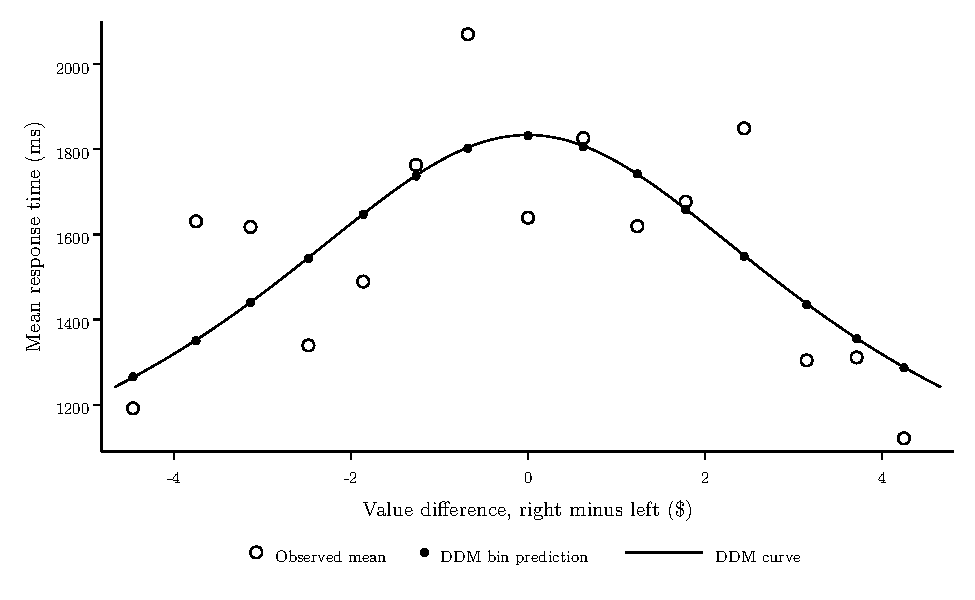
\includegraphics[width=0.94\textwidth]{fig-individual-response-time.pdf}
  \floatnotes{Source: \texttt{indv-Data.csv}, UNI \texttt{ts3686};
  \RTKept\ trials within two standard deviations of the full-sample mean.
  Open circles show $T_j$; black dots show $\widehat A g_j+\widehat t_0$.
  The curve is equation~\eqref{eq:mean-time} evaluated at $d$.
  The bin boundaries, $d_j$, and $\widehat\alpha$ are held fixed from
  the choice analysis; both $T_j$ and $g_j$ average over retained trials.}
\end{figure}

\subsection{Assessment}
At large bid differences, I usually choose quickly (Figure~\ref{fig:individual-time}).
Near equal bids, the pattern is less regular. The slowest bin, near $d_j=-0.68$,
averages 2,070 milliseconds; the next, with nearly equal bids, averages 1,639.
I may have found similarly valued snacks easy to choose between, but the pairs
near $d_j=-0.68$ harder despite their larger bid gaps.

The bin near $d_j=2.45$ also stands out. Its mean of 1,849 milliseconds
exceeds the fitted value by about 301 milliseconds.
Across the 15 means, the model explains 55.4 percent of the variation, with
a root mean squared error (RMSE) of \RTRMSEIndividual\ milliseconds.


\section{Pooled Class Results}
\label{sec:pooled}

\subsection{Choice Probabilities (3a)}
The pooled data contain 30,450 choices, with $n_j$ right choices and $m_j$
left choices in bin $j$. Treating the supplied mean $d_j$ as each trial's
value difference gives the approximate log likelihood
\begin{equation}\label{eq:pooled-likelihood}
  LL_c(\alpha)
  \;=\;\sum_{j=1}^{15}
  \left[n_j\log P_\alpha(d_j)+m_j\log P_\alpha(-d_j)\right].
\end{equation}
Binomial coefficients can be omitted because they do not depend on $\alpha$.
The subscript $c$ denotes the class data. Maximizing
equation~\eqref{eq:pooled-likelihood} gives $\widehat\alpha_c=\AlphaPooled$, with
$LL_c(\widehat\alpha_c)=\LLPooled$.

The plotted frequencies are $p_j=n_j/(n_j+m_j)$ and
$e_j=P_{\widehat\alpha_c}(d_j)$. Under the bin-mean assumption,
$P_{\widehat\alpha_c}^{-1}(e_j)=d_j$ exactly, so the supplied means are also
the inverse-probability coordinates used in Question 1(d).

\begin{figure}[!ht]
  \centering
  \caption{\capttitle{Pooled Choice Frequencies}}
  \label{fig:pooled-choice}
  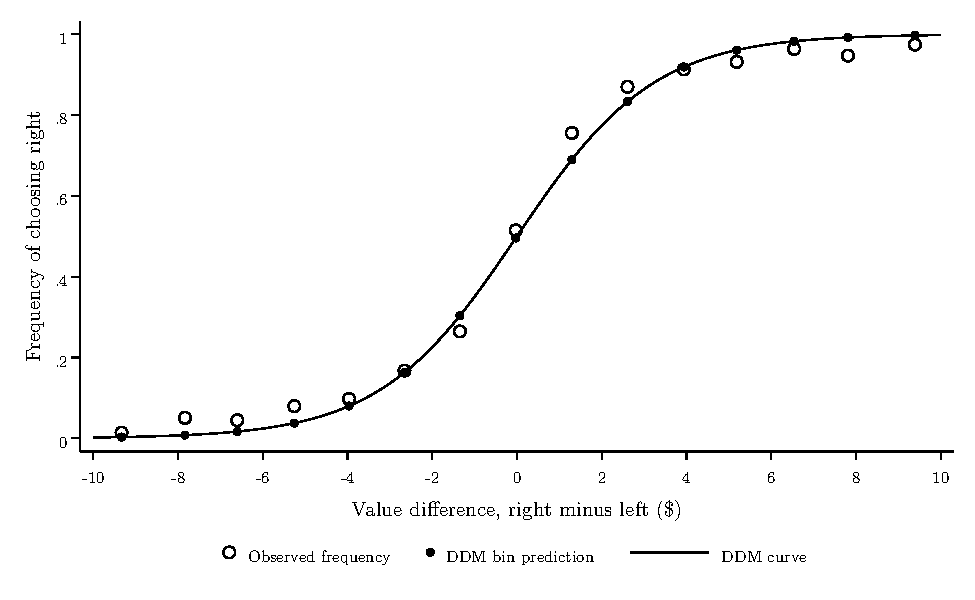
\includegraphics[width=0.94\textwidth]{fig-pooled-choice.pdf}
  \floatnotes{Source: \texttt{popData.csv}; 30,450 choices in 15 supplied bins.
  Open circles show $n_j/(n_j+m_j)$; black dots and the curve show
  predictions using the class estimate of alpha.
  Estimation treats each bin's supplied mean value difference as the value
  difference on every trial in that bin.}
\end{figure}

\begingroup
\clubpenalty=10000
The class choice fit has a count-weighted RMSE of \ChoiceRMSEPooled\ percentage
points (Figure~\ref{fig:pooled-choice}). The errors are systematic.
Near $d_j=-1.35$ and $d_j=1.29$, observed right-choice shares
are 26.5 and 75.6 percent; the fitted shares, 30.4 and 69.0 percent, lie
closer to one-half. This pattern reverses in the tails. Even with a value
advantage of \$7.81, the right snack was passed over in 5.3 percent of choices,
against just 0.8 percent predicted. A single $\alpha$ cannot match both the
steep change around equal bids and the less extreme choices in the tails.
\par
\endgroup

\subsection{Mean Response Times (3b)}
The pooled file contains only bin means, so individual outliers cannot be trimmed.
With $\widehat\alpha_c$ fixed, I regress $T_j$ on
$g_j=G_{\widehat\alpha_c}(d_j)$, giving each of the 15 bins equal weight.
The estimates are
\[
  \widehat A_c=\TimeScalePooled,
  \qquad \widehat t_{0,c}=\OffsetPooled\ \text{ms},
  \qquad R^2=\RSquaredPooled.
\]

\begin{figure}[!ht]
  \centering
  \caption{\capttitle{Pooled Mean Response Times}}
  \label{fig:pooled-time}
  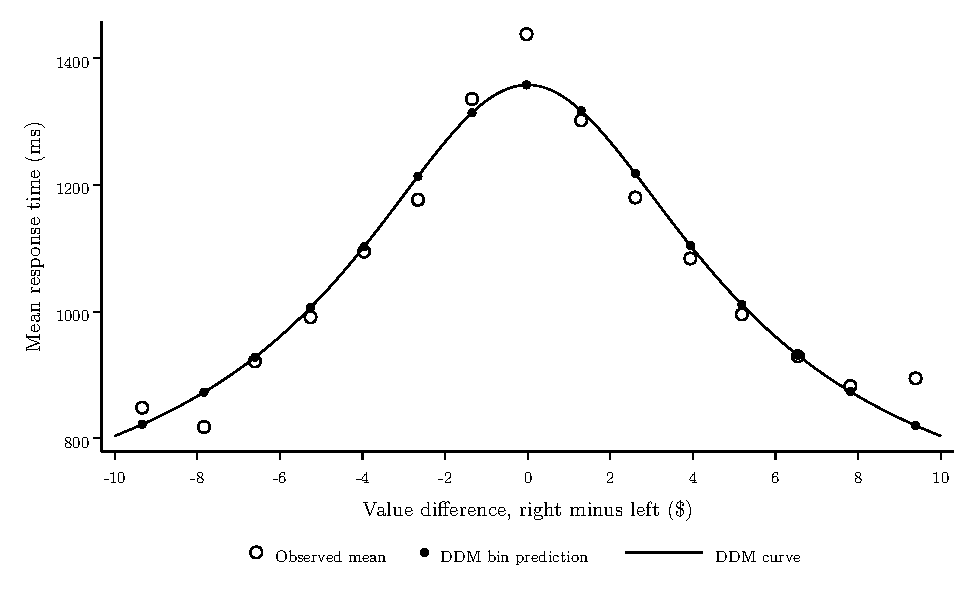
\includegraphics[width=0.94\textwidth]{fig-pooled-response-time.pdf}
  \floatnotes{Source: \texttt{popData.csv}; 15 supplied response-time means,
  in milliseconds. Open circles show $T_j$; black dots show
  $\widehat A_c g_j+\widehat t_{0,c}$.
  The time function uses the class estimate of alpha, and all bins receive
  equal OLS weight. Under the imposed bin-mean
  approximation, the black dots lie exactly on the theoretical curve.}
\end{figure}

The class means closely follow the predicted inverted-U
(Figure~\ref{fig:pooled-time}). Their RMSE is
\RTRMSEPooled\ milliseconds, compared with \RTRMSEIndividual\ milliseconds
for my data; $R^2$ is 0.961 (Table~\ref{tab:estimates}).

The largest residual is in the bin near $d_j=-0.03$, whose mean of
1,438 milliseconds exceeds the fitted value by about 80 milliseconds.
At the far right, the class also takes about 74 milliseconds longer
than predicted.

\begin{table}[!ht]
  \centering
  \caption{\capttitle{Estimated Parameters and Descriptive Fit}}
  \label{tab:estimates}
  \small
  \begin{tabular}{@{}lrr@{}}
    \toprule
    & Individual & Pooled class \\
    \midrule
    Choice trials &       435 &    30,450 \\
Choice sensitivity & 0.408351 & 0.308202 \\
Log likelihood & \(    -192.608\) & \(-14{,}580.856\) \\
Choice RMSE (percentage points) &   6.70 &   3.64 \\
\midrule
Response-time bins & 15 & 15 \\
Time scale, $\widehat{A}$ &  2,913.033 &  2,656.594 \\
Nondecision time, $\widehat{t}_0$ (ms) &    644.123 &    539.137 \\
\(R^2\) of bin means & 0.5542 & 0.9607 \\
Response-time RMSE (ms) &   172.21 &    36.71 \\
\bottomrule

  \end{tabular}
  \floatnotes{Choice estimates $\widehat\alpha$ (individual) and
  $\widehat\alpha_c$ (class) use maximum likelihood with no intercept.
  Response-time estimates use unweighted OLS on 15 means, holding the
  relevant choice estimate fixed. Individual response-time means use
  \RTKept\ retained trials; pooled means are used as supplied.
  Choice RMSE is $[\sum_j N_j(p_j-e_j)^2/\sum_jN_j]^{1/2}$,
  with $N_j$ the total choice count in a bin. Time RMSE divides the
  residual sum of squares by 15. $\alpha$ is in inverse dollars and
  $A$ is in milliseconds times dollars.}
\end{table}


\clearpage
\section{Conclusion}
\label{sec:conclusion}

The DDM fits the class's response-time curve more closely than my own.
My choices are relatively sensitive to bid differences, yet the bins where
I take longest are not those with the closest bids. This matters because
the time curve uses the sensitivity estimated from choices; changing $A$
and $t_0$ cannot move its peak away from equal values. The class means do
peak near equal bids.

Both fits depend on how well the bids measure value at the moment of choice.
Bids may contain noise or reflect values that changed before the choice
task. In the pooled data, averaging across students with different choice
sensitivities could also help explain a steeper center and less extreme
tails than a single logistic curve predicts. The close fit to class
response times does not establish that everyone shares the same
$\alpha$, $A$, and $t_0$.


% ============================================================
%  BIBLIOGRAPHY
% ============================================================

\newpage
\phantomsection
\printbibliography[heading=bibintoc,title={References}]

% ============================================================
%  APPENDIX
% ============================================================

\newpage
\appendix
\appendixnumbering
\doublespacing

\section{Bin Calculations}
\label{app:bin-results}

Tables~\ref{tab:individual-bins} and~\ref{tab:pooled-bins} report the
quantities plotted in the four figures. The Stata and Python code that
produces them, together with a standalone replication package, is at
\href{\paperrepourl}{\nolinkurl{\paperlatesttext}}.

\begin{table}[H]
  \centering
  \caption{\capttitle{Individual Bin Calculations}}
  \label{tab:individual-bins}
  \small
  \setlength{\tabcolsep}{4pt}
  \begin{tabular}{@{}rrrrrrrrr@{}}
    \toprule
    Bin & $d_j$ & $N_j$ & $N_j^{RT}$ & $p_j$ & $e_j$ & $g_j$
        & $T_j$ & $\widehat T_j$ \\
    \midrule
     1 & \(-4.459\) &    5 &    4 & 0.000 & 0.026 & 0.2133 &  1191.5 &  1265.4 \\
 2 & \(-3.747\) &   25 &   25 & 0.040 & 0.045 & 0.2425 &  1630.8 &  1350.6 \\
 3 & \(-3.132\) &   34 &   34 & 0.118 & 0.072 & 0.2731 &  1617.6 &  1439.8 \\
 4 & \(-2.477\) &   34 &   33 & 0.029 & 0.117 & 0.3087 &  1339.3 &  1543.3 \\
 5 & \(-1.858\) &   34 &   33 & 0.088 & 0.180 & 0.3443 &  1489.3 &  1647.1 \\
 6 & \(-1.261\) &   34 &   33 & 0.235 & 0.263 & 0.3752 &  1763.1 &  1737.1 \\
 7 & \(-0.675\) &   34 &   33 & 0.382 & 0.366 & 0.3977 &  2070.4 &  1802.7 \\
 8 & \( 0.004\) &   34 &   31 & 0.529 & 0.501 & 0.4079 &  1639.2 &  1832.3 \\
 9 & \( 0.628\) &   34 &   31 & 0.647 & 0.625 & 0.3988 &  1826.3 &  1805.7 \\
10 & \( 1.239\) &   34 &   30 & 0.588 & 0.733 & 0.3770 &  1619.3 &  1742.5 \\
11 & \( 1.785\) &   34 &   34 & 0.706 & 0.811 & 0.3480 &  1676.9 &  1657.9 \\
12 & \( 2.445\) &   35 &   34 & 0.829 & 0.880 & 0.3104 &  1849.3 &  1548.4 \\
13 & \( 3.151\) &   34 &   33 & 0.941 & 0.929 & 0.2714 &  1304.1 &  1434.8 \\
14 & \( 3.716\) &   25 &   25 & 1.000 & 0.954 & 0.2440 &  1311.0 &  1354.9 \\
15 & \( 4.251\) &    5 &    5 & 1.000 & 0.970 & 0.2207 &  1121.0 &  1286.9 \\
\bottomrule

  \end{tabular}
  \floatnotes{$N_j$ counts all choices; $N_j^{RT}$ counts retained
  response-time trials. $p_j$ and $e_j$ use all choices, while $T_j$ and
  $g_j$ use retained trials. $\widehat T_j=\widehat A g_j+\widehat t_0$.
  $d_j$ is in dollars and both time columns are in milliseconds.
  Source: \texttt{indv-Data.csv}, UNI \texttt{ts3686}.}
\end{table}

\subsection{Averaging Convention}
Both $g_j$ and $T_j$ use the \RTKept\ retained response-time trials.
Averaging $G_{\widehat\alpha}$ over all original trials instead gives
$\widehat A=\AltAIndividual$, $\widehat t_0=\AltOffsetIndividual$
milliseconds, and $R^2=\AltRSquaredIndividual$.

The fitted individual points use the mean of $G_{\widehat\alpha}$ within
each bin, while the smooth curve evaluates it at $d_j$. The nonlinearity
makes the two differ slightly; their maximum vertical separation is
\CurveGapIndividual\ milliseconds.

\begin{table}[H]
  \centering
  \caption{\capttitle{Pooled Bin Calculations}}
  \label{tab:pooled-bins}
  \small
  \setlength{\tabcolsep}{5pt}
  \begin{tabular}{@{}rrrrrrrr@{}}
    \toprule
    Bin & $d_j$ & $n_j+m_j$ & $p_j$ & $e_j$ & $g_j$
        & $T_j$ & $\widehat T_j$ \\
    \midrule
     1 & \(-9.3315\) &    72 & 0.014 & 0.003 & 0.1065 &   848.3 &   822.0 \\
 2 & \(-7.8358\) &   217 & 0.051 & 0.008 & 0.1256 &   817.8 &   872.8 \\
 3 & \(-6.6015\) &   424 & 0.045 & 0.017 & 0.1464 &   921.6 &   928.0 \\
 4 & \(-5.2565\) & 1,193 & 0.080 & 0.038 & 0.1759 &   991.2 &  1006.4 \\
 5 & \(-3.9613\) & 2,235 & 0.098 & 0.080 & 0.2120 &  1094.8 &  1102.4 \\
 6 & \(-2.6560\) & 3,552 & 0.168 & 0.163 & 0.2539 &  1176.6 &  1213.6 \\
 7 & \(-1.3475\) & 4,697 & 0.265 & 0.304 & 0.2916 &  1335.8 &  1313.9 \\
 8 & \(-0.0281\) & 5,439 & 0.515 & 0.496 & 0.3082 &  1438.0 &  1357.9 \\
 9 & \(1.2947\) & 4,770 & 0.756 & 0.690 & 0.2928 &  1302.1 &  1317.0 \\
10 & \(2.6073\) & 3,649 & 0.870 & 0.833 & 0.2554 &  1180.2 &  1217.8 \\
11 & \(3.9377\) & 2,263 & 0.913 & 0.919 & 0.2128 &  1083.9 &  1104.3 \\
12 & \(5.1851\) & 1,198 & 0.932 & 0.961 & 0.1777 &   995.8 &  1011.2 \\
13 & \(6.5403\) &   438 & 0.963 & 0.983 & 0.1476 &   929.6 &   931.2 \\
14 & \(7.8100\) &   226 & 0.947 & 0.992 & 0.1260 &   882.4 &   873.8 \\
15 & \(9.3905\) &    77 & 0.974 & 0.997 & 0.1058 &   894.7 &   820.3 \\
\bottomrule

  \end{tabular}
  \floatnotes{The supplied $d_j$ is an arithmetic mean, used as the common
  value difference for every trial in its bin. The time function is evaluated
  at $d_j$ using the class estimate of alpha to give $g_j$;
  $\widehat T_j=\widehat A_c g_j+\widehat t_{0,c}$.
  $d_j$ is in dollars and both time columns are in milliseconds.
  Source: \texttt{popData.csv}.}
\end{table}


\end{document}
